\chapter{Discussion}
Please tell more about conclusion and how to the next work of this study.

\section{Aip Suprapto Munari/1164063}
\subsection{Teori}
\begin{enumerate}
\item Mengapa file suara harus dilakukan MFCC, dilengkapi dengan ilustrasi atau gambar.

Mel Frequency Cepstral Coefficients (MFCC) merupakan koefisien yang merepresentasikan audio. Sehingga diharuskannya melakukan MFCC kepada objek suara atau audio agar suara dapat berubah atau diubah ke dalam bentuk data matrix dimana telah dilakukan ekstraksi oleh MFCC kemudian direalisasikan sebagai data matrix.

\begin{itemize}
\item Ilustrasi Gambar:

\begin{figure}[ht]
\centering
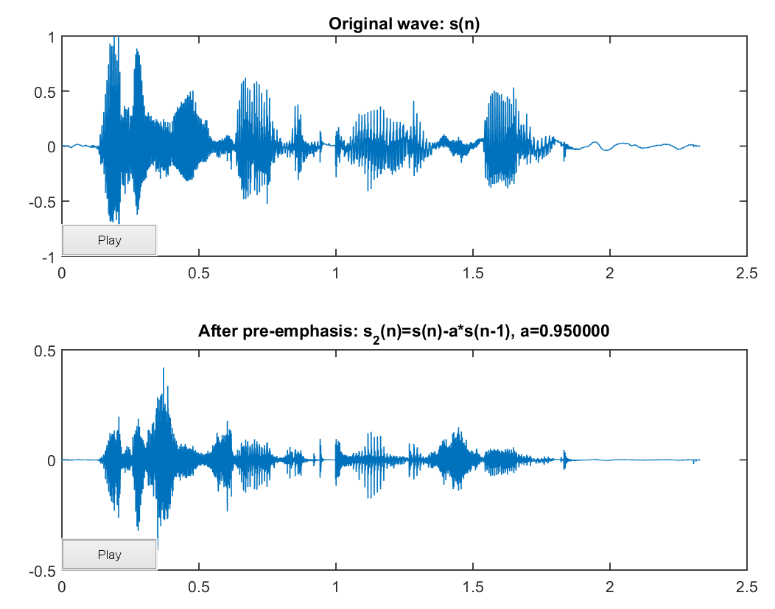
\includegraphics[scale=0.7]{figures/AIP/f1.PNG}
\caption{MFCC - Aip}
\label{MFCC - Aip}
\end{figure}

\end{itemize}

\item Konsep dasar Neural Network, dilengkapi dengan ilustrasi atau gambar.

Neural Network merupakan replika dari sistem syaraf yang terdapat pada sistem otak manusia. Dalam proses kerjanya, otak manusia disusun atas miliaran neuron dimana setiap neuron akan terhubung pada puluhan ribu neuron lain.
\begin{itemize}
\item Ilustrasi Gambar:

\begin{figure}[ht]
\centering
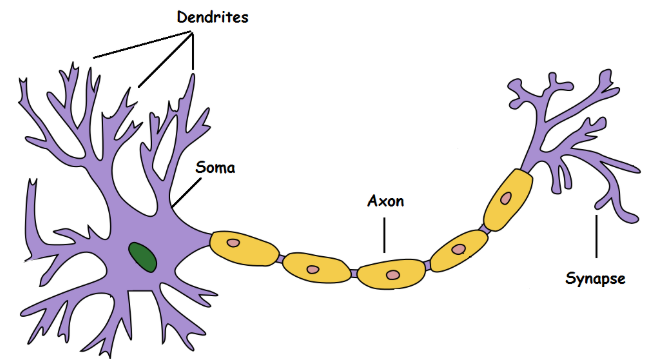
\includegraphics[scale=0.7]{figures/AIP/f2.PNG}
\caption{Konsep Dasar Neural Network - Aip}
\label{Konsep Dasar Neural Network - Aip}
\end{figure}

\end{itemize}

\item Konsep pembobotan Neural Network, dilengkapi dengan ilustrasi atau gambar.

Bobot merupakan suatu nilai yang mendefinisikan tingkat atau kepentingan hubungan antara suatu node dengan node yang lain. Semakin besar bobot suatu hubungan menandakan semakin pentingnya hubungan kedua node tersebut. Bobot merupakan suatu hubungan berupa bilangan real maupun integer, tergantung dari jenis permasalahan dan model yang digunakan. Bobot-bobot tersebut bisa ditentukan untuk berada didalam interval tertentu. selama proses pelatihan, bobot tersebut dapat menyesuaikan dengan pola-pola input.

\begin{itemize}
\item Ilustrasi Gambar :

\begin{figure}[ht]
\centering
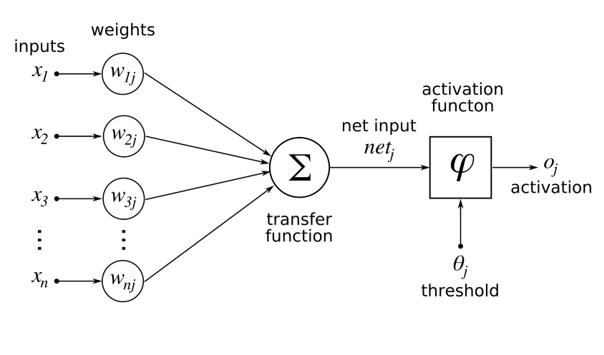
\includegraphics[scale=0.7]{figures/AIP/f3.PNG}
\caption{Konsep Pembobotan Neural Network - Aip}
\label{Konsep Pembobotan Neural Network - Aip}
\end{figure}

\end{itemize}

\item Konsep fungsi aktifasi dalam Neural Network, dilengkapi dengan ilustrasi atau gambar.
Operasi matematik yang dikenakan pada sinyal output y. Sehingga fungsi ini akan digunakan untuk pengaktifan dan juga penonaktifan neuron.
\begin{itemize}
\item Dalam konsep fungsi aktivasi Neuron Network terdapat beberapa jenis:
\begin{itemize}
\item Fungsi Undak Biner Hard Limit ( Menkonversi nilai masukan dari suatu variabel )
\item Fungsi Undak Biner Threshold ( Menggunakan nilai ambang 0 sebagai batas eksekusil )
\item Fungsi Bipolar Symetric Hard Limit ( Mempunyai keluaran bernilai 1 dan 0 )
\item Fungsi Bipolar Threshold ( Mempunyai keluaran bernilai 1, 0 atau -1 )

\item Ilustrasi Gambar:

\begin{figure}[ht]
\centering
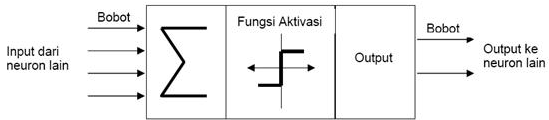
\includegraphics[scale=0.7]{figures/AIP/f4.PNG}
\caption{Konsep Fungsi Aktifasi - Aip}
\label{Konsep Fungsi Aktivasi - Aip}
\end{figure}

\end{itemize}
\end{itemize}

\item Cara membaca hasil plot dari MFCC, dilengkapi dengan ilustrasi atau gambar.

Penjelasan Cara Membaca Hasil Plot Dari MFCC :
\begin{itemize}
\item Ilustrasi Gambar :
\begin{figure}[ht]
\centering
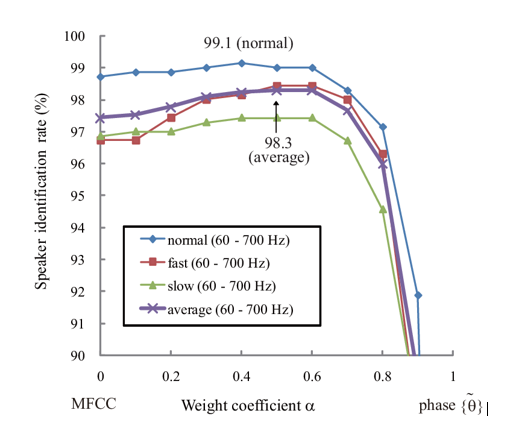
\includegraphics[scale=0.4]{figures/AIP/f5.PNG}
\caption{Plot MFCC - Aip}
\label{Plot MFCC - Aip}
\end{figure}

\end{itemize}

\item Apa itu One-Hot Encoding, dilengkapi dengan ilustrasi atau gambar.


One-Hot Encoding adalah sekelompok bit yang kombinasi hukumnya hanya terdiri dari bit dengan bit tinggi (1) dan bit lainnya rendah (0). Implementasi serupa di mana semua bit '1' kecuali satu '0' kadang-kadang disebut one-cold. Dalam statistik, variabel dummy mewakili teknik serupa untuk mewakili data kategorikal.
\begin{itemize}
\item Ilustrasi Gambar:

\begin{figure}[ht]
\centering
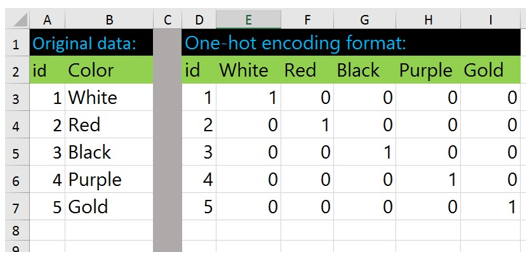
\includegraphics[scale=0.4]{figures/AIP/f6.PNG}
\caption{One-Hot Encoding - Aip}
\label{One-Hot Encoding - Aip}
\end{figure}

\end{itemize}

\item Fungsi dari np.unique dan to.categorical, dilengkapi dengan ilustrasi atau gambar.
\begin{enumerate}
\item np.unique:

Berfungsi untuk menemukan elemen unik array. Ada tiga output opsional selain elemen unik:

\begin{itemize}
\item Indeks array input yang memberikan nilai unik
\item Indeks array unik yang merekonstruksi array input
\item Berapa kali setiap nilai unik muncul dalam array input
\end{itemize}

\item Ilustrasi Gambar :

\begin{figure}[ht]
\centering
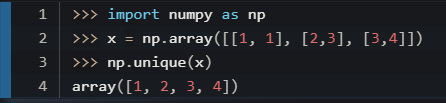
\includegraphics[scale=0.7]{figures/AIP/f7.PNG}
\caption{np.unique - Aip}
\label{np.unique - Aip}
\end{figure}

\item to.categorical:

Berfungsi untuk mengubah vektor kelas yang berupa integer menjadi matriks kelas biner.

\begin{itemize}
\item Ilustrasi Gambar :

\begin{figure}[ht]
\centering
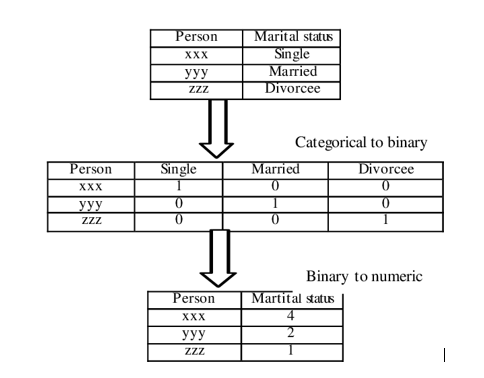
\includegraphics[scale=0.7]{figures/AIP/f7-2.png}
\caption{to.categorical - Aip}
\label{to.categorical - Aip}
\end{figure}

\end{itemize}
\end{enumerate}

\item Fungsi dari Sequential, dilengkapi dengan ilustrasi atau gambar.
Sebuah jenis model yang digunakan dalam perhitungan ataupun code program yang direalisasikan.
\begin{itemize}
\item Ilustrasi Gambar:

\begin{figure}[ht]
\centering
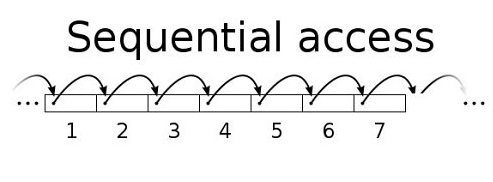
\includegraphics[scale=0.7]{figures/AIP/f8.PNG}
\caption{Sequential - Aip}
\label{Sequential - Aip}
\end{figure}

\end{itemize}
\end{enumerate}
